\documentclass{beamer}

\usetheme{Madrid}
% \usepackage{algpseudocode}

\usepackage{amsmath, amsfonts, amssymb, amsthm}
\usepackage[
    lmargin=3.7cm,%
	rmargin=2.5cm,%
	bmargin=2.5cm,%
	tmargin=2.5cm %
]{geometry}
\usepackage{graphicx}
\usepackage{float}
\usepackage{apalike}
\usepackage{hyperref}

\graphicspath{ {../images} }

%%%%%% ---- Theorem Styles and environments ----------------------
\theoremstyle{definition}
\newtheorem{thm}{Theorem}[section]
\newtheorem{defn}{Definition}[section]
\newtheorem*{notn}{Notation}


%%%%% ----- Custom Commands ----------------------
\newcommand{\ra}{\rightarrow} %% Shprt arrow to the right
\newcommand{\lra}{\longrightarrow}  %% long arrow to the right
\newcommand{\disp}{\displaystyle} %% for inline math displaystyle
\newcommand{\QQ}{\mathbb{Q}} %% Set of rational numbers
\newcommand{\NN}{\mathbb{N}} %% Set of natural numbers
\newcommand{\CC}{\mathbb{C}} %% Set of complex numbers
\newcommand{\RR}{\mathbb{R}} %% Set of real numbers
\newcommand{\htp}[1]{\underset{#1}{\simeq}} %%% Homotopy of two functions in


\title{Topology of Motion Planning Algorithms}
\author{Abdulrasheed Fawole}




\begin{document}

\begin{frame}
    \maketitle
\end{frame}

\begin{frame}
    \frametitle{Outline}

    \tableofcontents

\end{frame}

\section{Introduction}
\begin{frame}{Robotics}
    \begin{defn}[Oxford Dictionary]
        A robot is a machine capable of carrying out a complex series of actions
        automatically, especially one programmable by a computer.
    \end{defn}
    \begin{figure}[H]
        \centering
        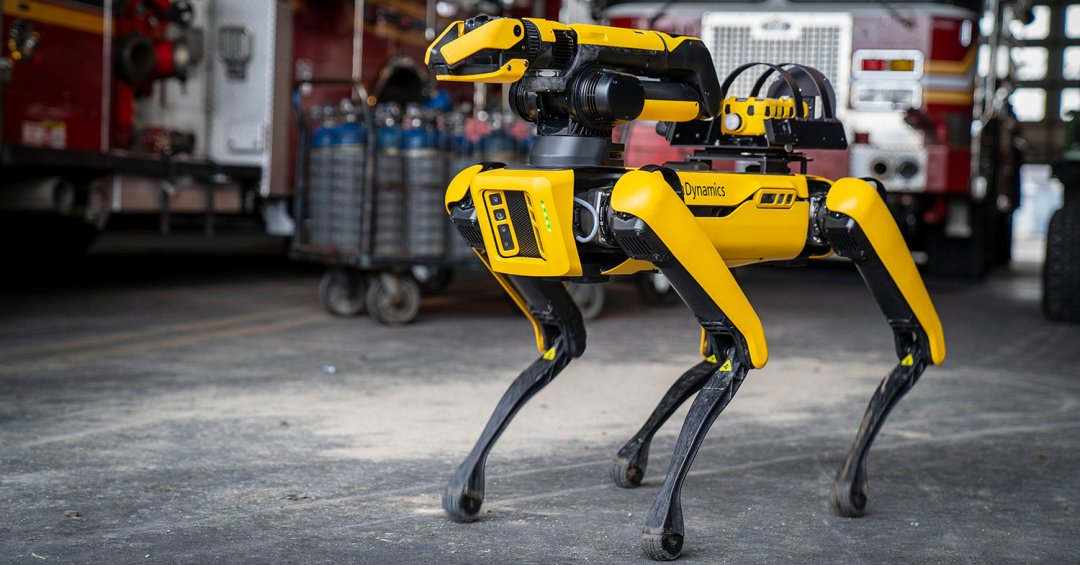
\includegraphics[scale=.25]{../images/boston-dynamics-spot}
        \caption[Boston dynamics robot (spot)]{Spot an agile multipurpose robot from Boston dynamics}
    \end{figure}
\end{frame}

\begin{frame}
    \frametitle{Application of Robotics}
    \begin{columns}[t]
        \begin{column}{.5\textwidth}
            \begin{figure}[H]
                \centering
                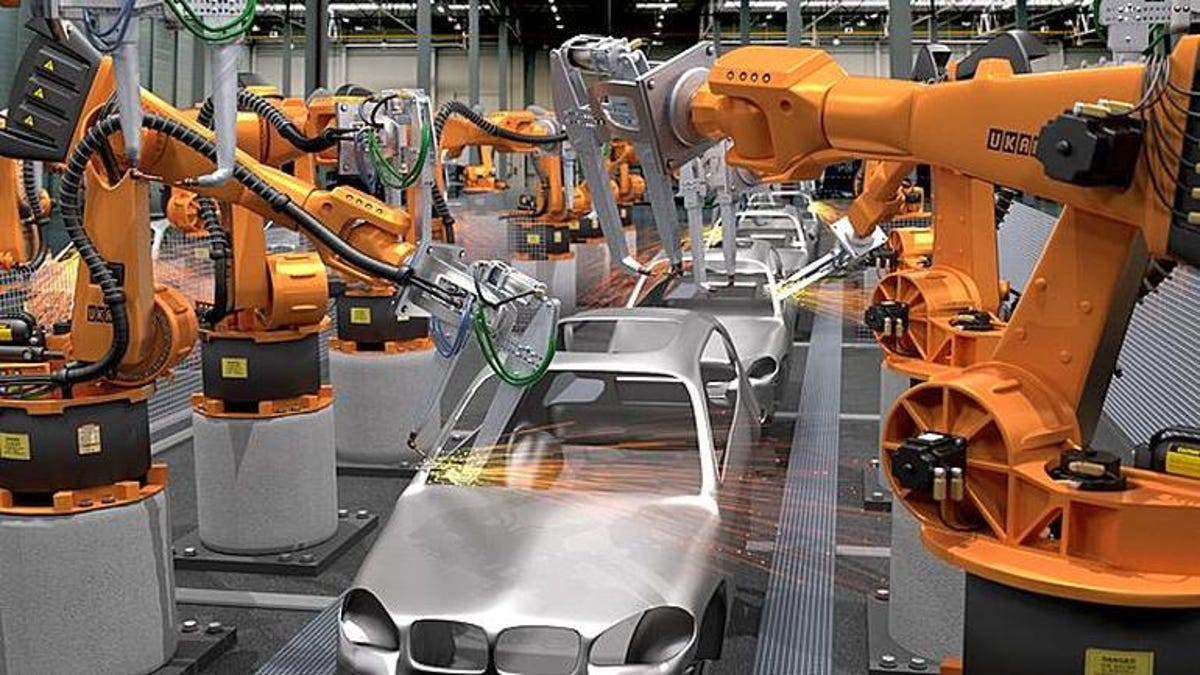
\includegraphics[width=\linewidth, height=.25\textheight, keepaspectratio]{../images/industral-robos.jpg}
                \caption[Boston dynamics robot (spot)]{Car Assembling}
            \end{figure}
            \begin{figure}[H]
                \centering
                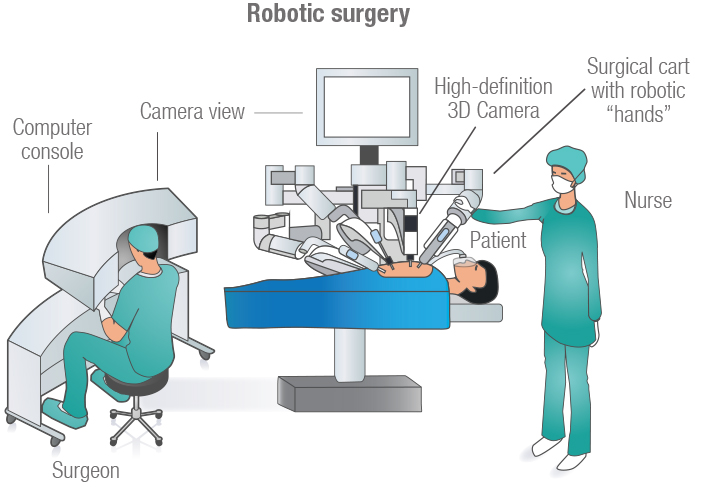
\includegraphics[width=\linewidth, height=.25\textheight, keepaspectratio]{../images/robotic-surgery-illustration.jpg}
                \caption[Boston dynamics robot (spot)]{Robotic Surgery}
            \end{figure}
        \end{column}

        \begin{column}{.5\textwidth}
            \begin{figure}[H]
                \centering
                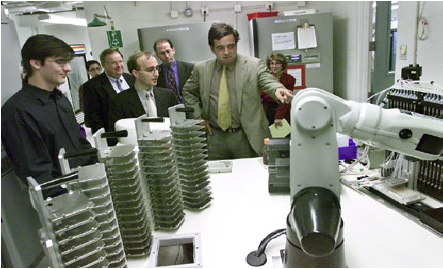
\includegraphics[width=\linewidth, height=.25\textheight, keepaspectratio]{../images/robo-lab.png}
                \caption[Boston dynamics robot (spot)]{Chemical and Bioolgy Labs}
            \end{figure}
            \begin{figure}[H]
                \centering
                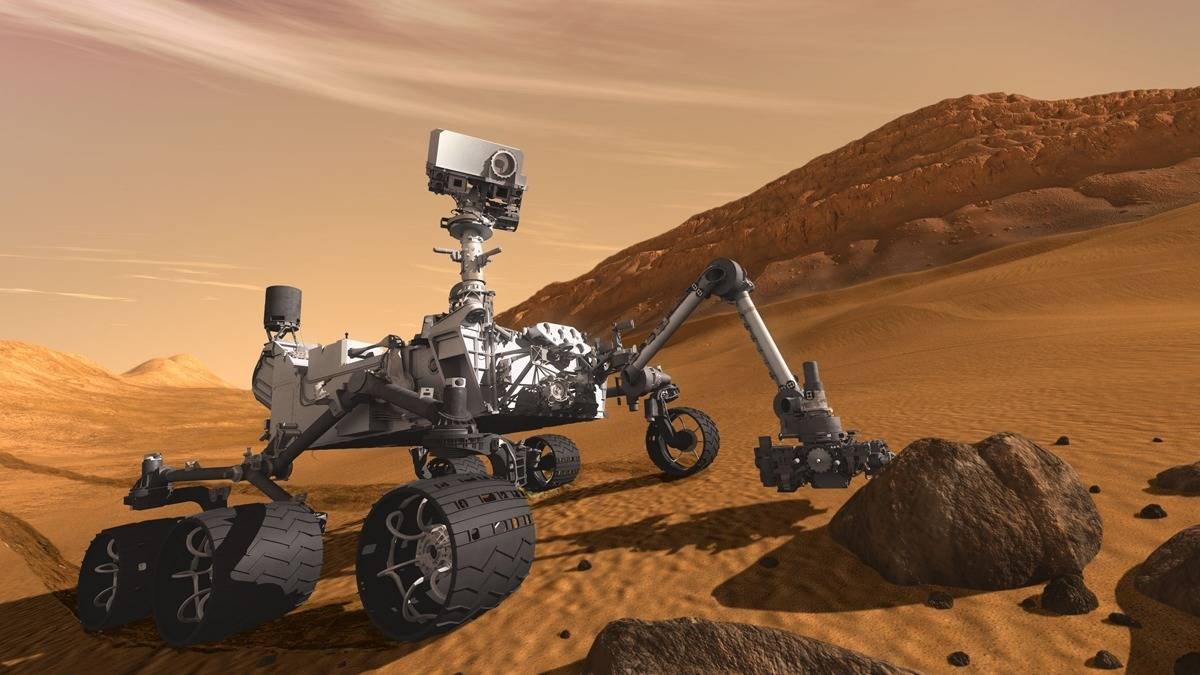
\includegraphics[width=\linewidth, height=.25\textheight, keepaspectratio]{../images/space-robots.jpg}
                \caption[Boston dynamics robot (spot)]{Space exploration}
            \end{figure}
        \end{column}

    \end{columns}
\end{frame}

\section{Literature Review}
\begin{frame}
    \frametitle{Literature Review}
    \begin{enumerate}
        \item Farber 2003 (Topological complexity)
        \item Farber and Grant 2007 (Symmetric Topological complexity)
        \item Derfoufi and Mamouni 2015 (Loop Motion Planning Algorithm)
        \item Derfoufi and Mamouni 2016 (String Topolocical Robotics)
        \item Pavesic 2018 (Instability of Robot Manipulator arm)
        \item Cohen et al 2021 (Motion Planning of multiple robots in 3D space)
    \end{enumerate}
\end{frame}

\section{Preliminaries}
\begin{frame}
    \frametitle{Preliminaries}
    \begin{defn}[Homotopy]
        Let $X$ and $Y$ be two topological spaces, let $f,g : X \lra Y$ be maps and $I = [0,1]$.
        Then the \textit{homotopy} from $f$ to $g$ is the map $F: X \times I \lra Y$ such that $F(x,0) = f(x)$ and $F(x,1) = g(x)$ for all points $x \in X$.
    \end{defn}
    For example, the function $H : \RR \times [0,1] \ra \RR^2$ given by $H (x,t) = \left(x, (1-t)x^3 + te^x\right)$ is a homotopy between the two maps $f,g : \RR \ra \RR^2$ given by $f(x) = (x, x^3)$ and $g(x) = (x, e^x)$

    \begin{defn}[Contractible space]
        A space $X$ is called contractible if the identity map $1_X$ is homotopic to the constant map at some point of $X$.
    \end{defn}
\end{frame}

\begin{frame}
    \frametitle{Preliminaries [Contd.]}
    \begin{defn}[Null-Homotopy]
        A function $f$ is said to be \textit{null-homotopic} if it is homotopic to a constant function.
    \end{defn}

    \begin{defn}[Homotopy Type]
        Two spaces $X$ and $Y$ have the same homotopy type (or are homotopy equivalent, or homotopic), if there exists maps $f: X \lra Y$ and $g : Y \lra X$
        % \begin{center}
        %     \begin{tikzcd}
        %         X \arrow[r, bend left=30, "f"]
        %         \arrow[r, "g"', leftarrow,bend right=30]
        %         & Y
        %     \end{tikzcd}
        % \end{center}
        such that $g \circ f \simeq 1_X$ and $f \circ g \simeq 1_X$
    \end{defn}

    \begin{defn}[Paracompact Space]
        $X$ is \textit{paracompact} if every open cover has a locally finite open refinement.
    \end{defn}
\end{frame}

\begin{frame}
    \frametitle{Preliminaries [Contd]}
    \begin{defn}[Lusternik-Schnirelmann category]
        Let $X$ be a topological space, the Lusternik-Schnirelmann category of $X$, denoted $\cat(X)$ is the smallest integer $k$ such that $X$ may be covered by $k$ open subsets
        \[
            V_1 \cup V_2 \cup \ldots \cup V_k = X
        \]
        with each inclusions $V_i \lra X$ null-homotopic.
    \end{defn}
    \begin{defn}[Configuration Space]
        The configuration space of a robot is a topological space, usually denoted $\cal{C}$ whose points parameterize the possible configurations of the robot.
    \end{defn}

\end{frame}

% \begin{frame}
%     \frametitle{Preliminaries [Contd]}

%     \begin{defn}[Zero-Divisors-Cup-Length, (Farber, 2003pp[])]
%         The kernel of the homomorphism (i.e the definition in equation \ref{cup:product}) will be called the ideal of zero-divisors of $H^*(X, \KK)$. The zero-divisors-cup-length, denoted $\zdcl$ of $H^*(X, \KK)$ is the length of the longest nontrivial product in the ideals of zero-divisors of $H^*(X, \KK)$.
%     \end{defn}

% \end{frame}

\section{Problem of Motion Planning}
\begin{frame}
    Find an algorithm which, given configurations $A$ and $B$ of the system, outputs a motion from $A$ to $B$.
    \frametitle{Problem of Motion Planning}
    \begin{figure}[H]
        \centering
        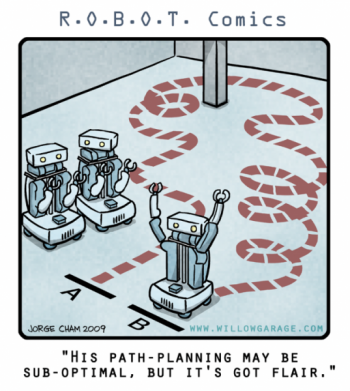
\includegraphics[scale=.3]{../images/planner.png}
    \end{figure}
    The topology of the configuration space $\mathcal{C}$ plays an important role. It dictates whether motion planning algorithms exist which are continuous in the input configurations.
\end{frame}

\begin{frame}
    \frametitle{Motion Planning Algorithm}
    \begin{defn}[Motion Planning Algorithm (Farber, 2003)]
        Let $X$ be a configuration space, the motion planning algorithm of a mechanical robot that moves in $X$ is given as an input and output as below:
        \begin{itemize}
            \item Input: a pair $(A,B)$ of two given points in the configuration space $X$
            \item Output: a continuus path from $A$ to $B$ aand hence a continuous section
                  \begin{align*}
                      s: X \times X \quad & \lra PX        \\
                      (A,B)               & \mapsto s(A,B)
                  \end{align*}
                  of the canonical projection
                  \begin{align*}
                      \pi: PX & \lra X \times X               \\
                      \gamma  & \mapsto (\gamma(0),\gamma(1))
                  \end{align*}
        \end{itemize}
    \end{defn}
\end{frame}

\section{Topological Complexity}

\begin{frame}
    \frametitle{Topolocical Complexity}
    \begin{defn}[Topological complexity, (Farber, 2003)]
        Given a path connected space $X$, we define the topological complexity of the motion planning in $X$ as the minimal number $\tcomp(X) = k$, such that the cartesian product $X \times X$ may be covered by $k$ open subsets
        \[
            X \times X  = U_1 \cup U_2 \cup \dots \cup U_k
        \]
        such that for any $i = 1,2, \ldots, k$ there exists a continuous motion planning $s_i: U_i \lra PX, \, \pi \circ s_i = 1_X$ over $U_i$. If no such $k$ exists we set $\tcomp(X) = \infty$.
    \end{defn}
\end{frame}

\begin{frame}
    \frametitle{Some Properties of $\tcomp(X)$}
    \begin{enumerate}
        \item If $X$ is a path-connected and paracompact space then,
              \begin{itemize}
                  \item \(
                        \cat(X) \le \tcomp(X) \le 2 \cdot \cat(X) - 1
                        \)
                  \item $\tcomp(X) \le 2 \cdot \dim(X) + 1$
              \end{itemize}
        \item $\tcomp(X) \ge \zdcl(H^*(X, \KK))$
        \item For any path-connected metric space $X$ and $Y$,
              \[
                  \tcomp(X \times Y) \le \tcomp(X) + \tcomp(Y) - 1
              \]
        \item If $X = \Sb^n$, that is an $n$-dimensional sphere then,
              \[
                  \tcomp(\Sb^n) = \begin{cases}
                      2, & \text{if $n$ is odd}  \\
                      3, & \text{if $n$ is even} \\
                  \end{cases}
              \]
    \end{enumerate}

\end{frame}

\begin{frame}
    \frametitle{Motion Planning of Robot Arm}
    \begin{thm}[Farber, 2003]
        Let $X  = \Sb^m \times \ldots \times \Sb^m$ be a cartesian product of $n$ copies of the $m-$-dimensional sphere $\Sb^m$. Then
        \[
            \tcomp(X) = \begin{cases}
                n + 1  & \text{if $m$ is odd}  \\
                2n + 1 & \text{if $m$ is even}
            \end{cases}
        \]
        \begin{figure}[h]
            \centering
            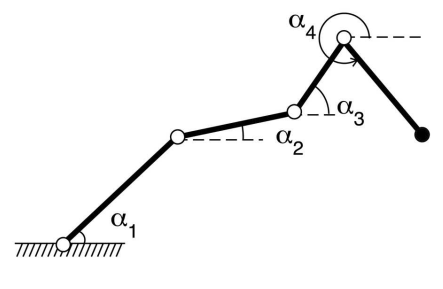
\includegraphics[scale=0.25]{../images/planar-robot-arm.png}
            \caption{Planar Robot Arm}
        \end{figure}
    \end{thm}
\end{frame}

\begin{frame}
    \frametitle{Motion Planning of Ronot Arm [Contd]}
    \textbf{Proof:}\\
    To show this result we firstly show that the LHS is less or equal to the RHS and also show otherwise too. To show the first inequality we use the method of induction. For the base case $n = 1$, the result holds by using property  4.

    Now suppose the inequality is true for all $n = k$, then we have the following
    \[
        \tcomp(X) = \begin{cases}
            k + 1  & \text{if $m$ is odd}  \\
            2k + 1 & \text{if $m$ is even}
        \end{cases}
    \]
    Let $X_k$ be the cartesian product of $k$ copies of the $m$-dimensional sphere, then by the product inequality property of $\tcomp(X)$ we have
    \[
        \tcomp(X_k \times \Sb^m) \le \tcomp(X_k) + \tcomp(\Sb^m) - 1
    \]
\end{frame}

\begin{frame}
    \frametitle{Motion Planning of Robot Arm [Contd]}
    then we have for odd $m,\, \tcomp(X_k \times \Sb^m) \le k +2$ and for even $m,\, \tcomp(X_k \times \Sb^m) \le 2k +3$, which shows our inductive step. Hence, showing the first inequality.

    Conversely, for the second inequality, let $a_i \in H^m(X, \QQ)$ denote the cohomology class which is the pull-back of the fundamental class of $\Sb^m$ under the projection $X \ra \Sb^m$ onto the $i$-th factor; for $i = 1, 2, \ldots, n$. We notice that
    \[
        \prod_{i=1}^{n} (1 \otimes a_i - a_i \otimes 1) \neq 0 \in H^*(X \times X, \QQ)
    \]
    This shows that $\zdcl(X)$ is at least $n$. If $m$ is even then
    \[
        \prod_{i=1}^{n} (1 \otimes a_i - a_i \otimes 1)^2 \neq 0 \in H^*(X \times X, \QQ)
    \]
    Hence for $m$ even, $\zdcl(X)$ is at least $2n$, applying property 2 completes the proof.
\end{frame}

\section{The Rapidly-exploring Random Tree (RRT) algorithm}

\begin{frame}
    \frametitle{The Rapidly-exploring Random Tree (RRT) algorithm}
    RRT algorithm is a sampling-based algorithm for path planning. The RRT algorithm starts with a tree of nodes, with the start node as the root node. Then, it iteratively samples a random point in the search space and connects it to the nearest node in the tree. If the new node is not in collision with any obstacles, it is added to the tree. The algorithm continues iterating until it finds a path from the start node to the goal node.

\end{frame}

\begin{frame}[fragile]
    \frametitle{RRT algorithm [Contd]}
    \begin{algorithm}[H]
        \caption{RRT (Rapidly-exploring Random Tree)}
        \begin{algorithmic}[1]
            \STATE Initialize a tree $T$ with the start node $s$.
            \FOR{each iteration}
            \STATE Sample a random point $q$ in the search space.
            \STATE Find the nearest node $n$ in $T$ to $q$.
            \STATE Steer $n$ towards $q$ to obtain a new node $m$.
            \IF{no collision between $m$ and obstacles}
            \STATE Add $m$ to $T$.
            \ENDIF
            \ENDFOR
            \STATE Return the path from $s$ to the goal node in $T$.
        \end{algorithmic}
    \end{algorithm}
\end{frame}

\begin{frame}
    \frametitle{RRT Algorithm [Contd]}
    For the RRT algorithm to be very useful in the world application it is implemented in softwares which power the different camera sensors, LIDAR and other perception sensors in mapping environment and planning the motion of a robot.
    \begin{figure}[h]
        \centering
        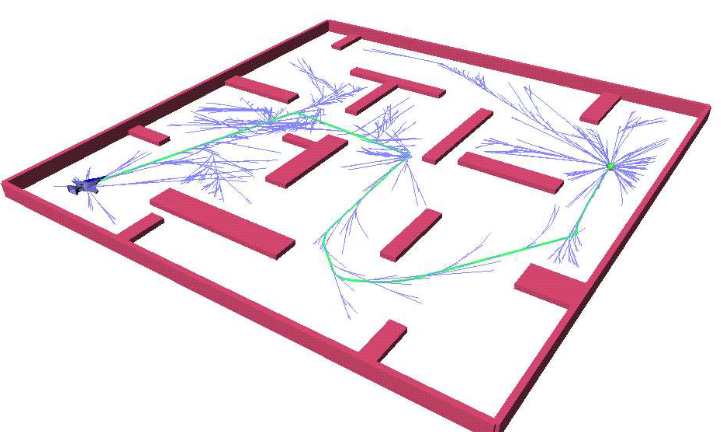
\includegraphics[scale=0.3]{../images/rrt1.png}
        \caption{RRTs of 13,600 nodes for the planar body with unilateral thrusters that allow it to rotate freely but translate only in the forward direction.}
    \end{figure}
\end{frame}


\begin{frame}
    \frametitle{Conclusion}
    Since cost optimality is always needed for the any robot motion planning algorithm, many variant has been improvised to improve more on the effectiveness of the RRT algorithm, and computational time has also been reduced with the new algorithms like RRT*, RRT*-smart, RRT-plus, etc.

    In conclusion, it has been show that the topological complexity that is the optimality of an algorithm is very important in the designing of motion planner for a robot and this also it also takes into consideration the configuration space, the obtacle space, etc, and the constraints on the paths such as weather condition, land structure, warehouse arrangments, etc presents in a robot workspace.
\end{frame}

\section{References}
\begin{frame}{References}
    \begin{enumerate}
        \item Derfoufi, Y. and Mamouni, M. I. (2015). Loop topological complexity. Bulletin to Computational Applied Mathematics, 3:31--36.
        \item Derfoufi, Y. and Mamouni, M. I. (2016). String topological robotics. JP Journal
        of Geometry and Topology, 19(3):189--208.
        \item Farber, M. (2003). Topological complexity of motion planning. Discrete and Computational Geometry, 29(2):211--221.
        \item Farber, M. and Grant, M. (2007). Symmetric motion planning. Contemporary Mathematics, 438:85--104. 
        \item James, I. M. (1978). On category, in the sense of lusternik-schnirelmann. Topology, 17(4):331--348.
        \item Mamouni, M. I. (2022). Pure and Applied Algebraic Topology. Cambridge Scholars Publishing.
        \item Pavesic, P. (2018). A topologist's view of kinematic maps and manipulation complexity. Contemp. Math, 702:61--83.
    \end{enumerate}
\end{frame}




\end{document}